\subsection{Présentation du lanceur SP02}
\label{sec:presentation_SP02}

\subsubsection{Cadre de lancement : le C’Space et ses contraintes}

Le développement du lanceur SP-02 s’inscrit dans le cadre de la campagne nationale \gls{C'Space}, organisée par
\gls{Planète Sciences} avec le soutien du \acrfull{CNES}. Cette campagne constitue aujourd’hui le principal, et pratiquement
l’unique, cadre de lancement accessible en France pour des projets de fusées expérimentales étudiantes. Elle fournit un
environnement réglementé permettant la réalisation d’essais en vol, sous réserve du respect d’un cahier des charges technique et
de sûreté particulièrement structurant.\\

La participation au \gls{C'Space} implique la conformité à un \acrfull{CDC} exigeant, couvrant notamment les aspects de sécurité
sol et vol, la robustesse des architectures retenues, la maîtrise des risques et la justification détaillée des choix techniques.
Les systèmes critiques du lanceur, en particulier ceux liés à la séparation d’étages, doivent ainsi faire l’objet d’analyses
documentées, d’essais préalables et d’une traçabilité complète. Certaines solutions, bien que pertinentes d’un point de vue
théorique ou industriel, peuvent se révéler difficilement compatibles avec ce cadre, notamment en raison des contraintes
réglementaires associées à l’utilisation de dispositifs pyrotechniques ou de mécanismes complexes.\\

Ce contexte impose également des contraintes fortes sur la philosophie de conception du lanceur. Le véhicule doit être
suffisamment simple et robuste pour garantir un niveau de sûreté acceptable, tout en restant instrumentable et exploitable du
point de vue expérimental. La reproductibilité des essais, la capacité à analyser les événements de vol et la récupération des
données constituent des critères déterminants dans l’évaluation des projets par les instances de suivi.\\

Ainsi, le cadre du \gls{C'Space} ne se limite pas à une opportunité de lancement, mais constitue un élément structurant de la
conception du lanceur SP-02. Les choix architecturaux retenus résultent directement de ce compromis entre exigences
réglementaires, contraintes opérationnelles et objectifs expérimentaux. La section suivante présente l’architecture générale du
lanceur SP-02, telle qu’elle a été définie pour répondre à ces contraintes tout en servant de support à l’étude de la séparation
d’étages assistée par aérofreinage.

\begin{figure}[h!]
    \centering
    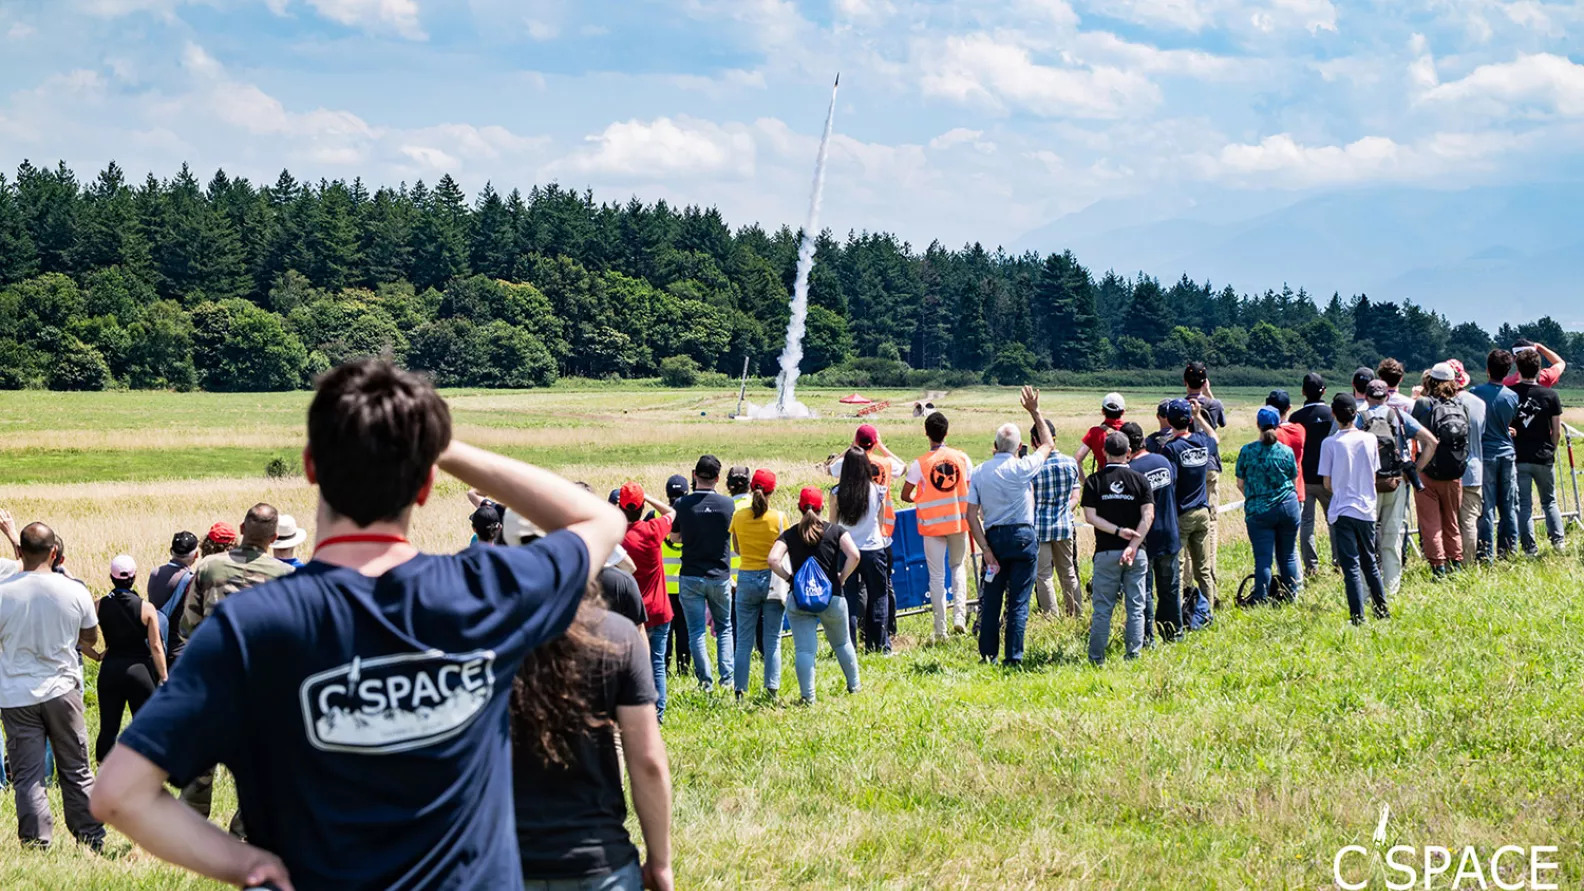
\includegraphics[width=0.7\textwidth]{figures/cspace-2024-1.jpg}
    \caption{Décollage d'une fusée expérimentale au C'Space 2024. \copyright CNES/C'Space/Thomas Labois}
\end{figure}

\subsubsection{Architecture générale du lanceur SP-02}

L’architecture repose sur une organisation claire en deux étages. Le premier étage assure la phase propulsive initiale et
constitue le support principal de l’expérience de séparation, en embarquant les dispositifs aérodynamiques étudiés. Le second
étage est un étage propulsif à part entière, permettant à la fois l’étude du comportement relatif lors de la séparation et la
poursuite du vol après celle-ci. Son intégration implique des fonctions spécifiques de commande et de sécurité liées à l’allumage
moteur, qui seront détaillées ultérieurement. Les architectures mécanique et électronique du lanceur SP-02 sont présentées dans les sections suivantes, dans la mesure
strictement nécessaire à la compréhension du principe étudié et des analyses menées par la suite.

\newpage

\subsubsubsection{Architecture mécanique}

Le premier étage du lanceur SP-02, d’une longueur totale de 1130 mm et d’un diamètre de 104 mm, est propulsé par un moteur
à ergole solide K570 - Pro54-5G, d'une poussée moyenne de 572 N, d'temps de combustion de 3.61~s et donc d'une impulsion totale de
2070 Ns, c'est un moteur de classe K. Le premier étage intègre également 4 surfaces aérodynamiques (ailerons) pour la stabilité en
vol, ainsi que 3 aérofreins déployables destinés à générer l’effort de séparation placé au dessus du moteur. Viens ensuite le bloc
de parachute assurant la récupération du premier étage, suivi du bloc électronique contenant l’ensemble des cartes de commande et
d’acquisition. Enfin, la partie haute du premier étage se caractérise par le système de séparation.

\begin{figure}[h!]
    \centering
    \begin{tikzpicture}
    
        \node at (0, 0) {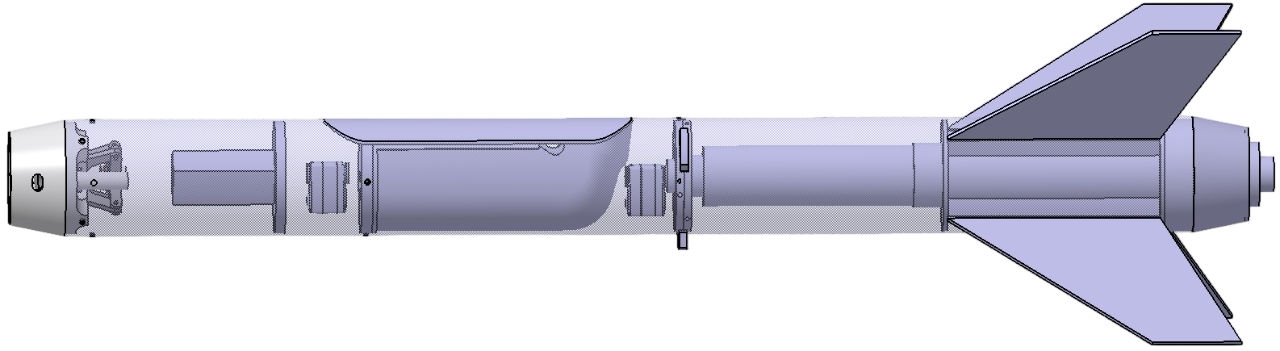
\includegraphics[width=\textwidth]{figures/catia_alpha.png}};
        
        \node (retreint_lbl)   at (+8.00, +2.5) {\textbf{Rétreint}};
        \node (bloc_propu_lbl) at (+4.30, +2.3) {\textbf{Bloc propulsion}};
        \node (propu_lbl)      at (+2.00, +1.5) {\textbf{Pro54-5G}};
        \node (aileron_lbl)    at (+2.00, -1.5) {\textbf{Ailerons (x4)}};
        \node (af_lbl)         at (+0.00, +2.3) {\textbf{Aérofreins (x3)}};
        \node (bloc_para_lbl)  at (-2.00, +1.5) {\textbf{Bloc parachute}};
        \node (bloc_elec_lbl)  at (-6.00, +2.3) {\textbf{Bloc électronique}};
        \node (bloc_sepa_lbl)  at (-6.00, -1.5) {\textbf{Bloc séparation}};

        \node (bloc_propu_box) at (+5.10, 0.00) [minimum width=35mm, minimum height=18mm, rectangle, line width=2, draw=red] {};
        
        \draw[red, ->, line width=1.5] (retreint_lbl.south)   -- (+7.20, +0.60);
        \draw[red, ->, line width=1.5] (bloc_propu_lbl.south) -- (bloc_propu_box.140);
        \draw[red, ->, line width=1.5] (propu_lbl.south)      -- (+2.20, +0.00);
        \draw[red, ->, line width=1.5] (aileron_lbl.east)     -- (+6.50, -1.50);
        \draw[red, ->, line width=1.5] (af_lbl.south)         -- (+0.30, +0.60);
        \draw[red, ->, line width=1.5] (bloc_para_lbl.south)  -- (-2.00, +0.00);
        \draw[red, ->, line width=1.5] (bloc_elec_lbl.south)  -- (-5.30, +0.00);
        \draw[red, ->, line width=1.5] (bloc_sepa_lbl.north)  -- (-7.30, +0.00);

    \end{tikzpicture}
    \caption{Vue du premier étage sur \acrshort{CATIA}}
    \label{fig:sp02_s1_ork}
\end{figure}

Le second étage, d’une longueur totale de 992 mm et d’un diamètre de 84 mm, est propulsé par un moteur 144G150 - Pro24-6G de la
même gamme que le moteur du premier étage. Il développe une poussée moyenne de 147~N pour un temps de combustion de 0.969~s, soit
une poussée totale de 144~Ns, c'est un moteur de classe G. Le second étage intègre une coiffe conique en tête faite en fibre de
verre et une pointe en aluminium, ainsi que 4 ailerons pour la stabilité en vol. Le bloc parachute assure la récupération de
l’étage, tandis que le bloc électronique contient les mêmes cartes que le premier étage afin de faciliter le développement. La
partie basse du second étage est quant à elle dédiée à l’interface de séparation avec le premier étage.

\begin{figure}[h]
    \centering
    \begin{tikzpicture}
    
        \node at (0, 0) {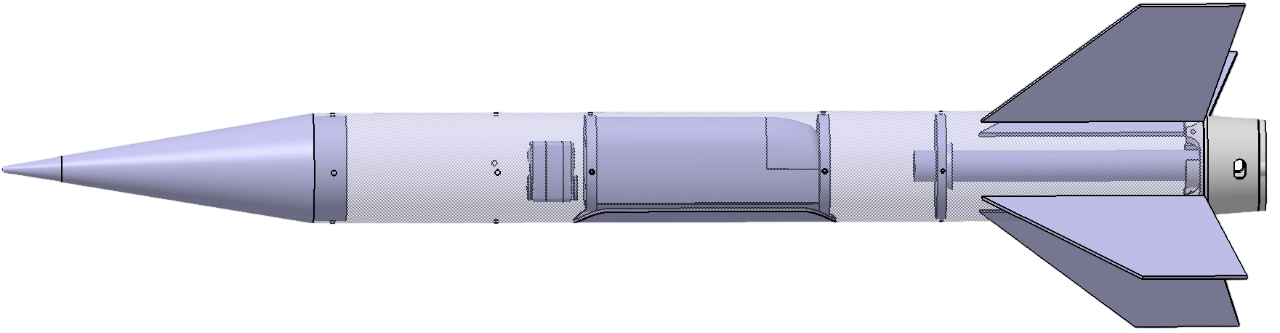
\includegraphics[width=\textwidth]{figures/catia_beta.png}};
        
        \node (bloc_sepa_lbl)   at (+8.00, +2.5) {\textbf{Interface de séparation}};
        \node (propu_lbl)       at (+4.30, +2.3) {\textbf{Pro24-6G}};
        \node (bague_propu_lbl) at (+3.00, +1.5) {\textbf{bague de centrage}};
        \node (aileron_lbl)     at (+2.00, -1.5) {\textbf{Ailerons (x4)}};
        \node (bloc_para_lbl)   at (+1.00, +2.3) {\textbf{Bloc parachute}};
        \node (bloc_elec_lbl)   at (-2.00, +1.5) {\textbf{Bloc électronique}};
        \node (coiffe_lbl)      at (-5.00, +2.3) {\textbf{Coiffe conique}};
        \node (pointe_alu_lbl)  at (-6.00, -1.5) {\textbf{Pointe aluminium}};

        \draw[red, ->, line width=1.5] (bloc_sepa_lbl.south)    -- (+7.40, +0.60);
        \draw[red, ->, line width=1.5] (propu_lbl.south)        -- (+5.20, +0.00);
        \draw[red, ->, line width=1.5] (bague_propu_lbl.south)  -- (+3.70, +0.00);
        \draw[red, ->, line width=1.5] (aileron_lbl.east)       -- (+6.50, -1.00);
        \draw[red, ->, line width=1.5] (bloc_para_lbl.south)    -- (+0.30, +0.60);
        \draw[red, ->, line width=1.5] (bloc_elec_lbl.south)    -- (-2.50, +0.00);
        \draw[red, ->, line width=1.5] (coiffe_lbl.south)       -- (-5.30, +0.00);
        \draw[red, ->, line width=1.5] (pointe_alu_lbl.north)   -- (-7.30, +0.00);

    \end{tikzpicture}
    \caption{Vue du second étage sur \acrshort{CATIA}}
    \label{fig:sp02_s2_ork}
\end{figure}

L'ensemble du lanceur SP-02 présente une longueur totale de 2062 mm et une masse théorique au décollage d'environs 9.3 kg, dont
6.9 kg pour le premier étage et 2.4 kg pour le second étage. 

\newpage

\subsubsubsection{Architecture électronique et instrumentation}

[ A FAIRE ]

\newpage

\subsubsection{Phase de vol}

Le vol de la fusée SP-02 se déroule selon six phases successives représentées dans la figure suivante. Ce découpage permet
d’identifier clairement les séquences critiques du lanceur et de situer la phase de séparation d’étages dans le contexte global
du vol.

\begin{figure}[h!]
    \centering
    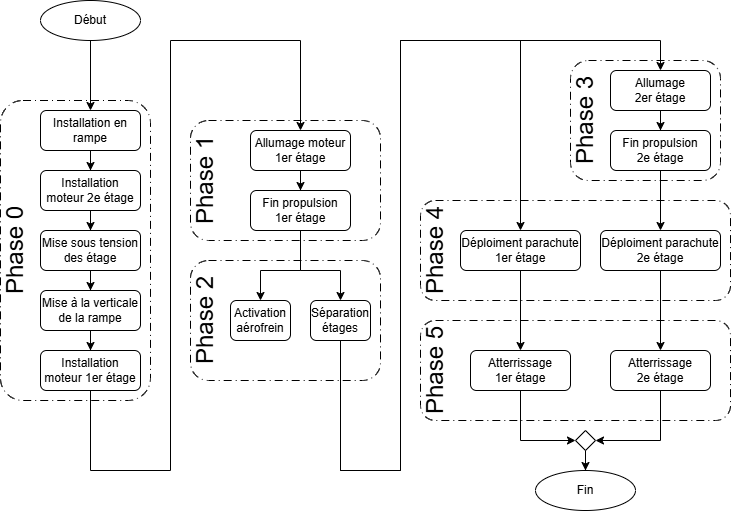
\includegraphics[width=\textwidth]{figures/Phase_vol.drawio.png}
    \caption{Phases de vol du lanceur SP-02}
    \label{fig:phases_vol_sp02}
\end{figure}

On distingue ainsi les phases suivantes :
\begin{itemize}
    \item \textbf{Phase 0 :} Préparation et mise en condition du système.
    \item \textbf{Phase 1 :} Propulsion et ascension du premier étage.
    \item \textbf{Phase 2 :} Séparation des étages.
    \item \textbf{Phase 3 :} Allumage et propulsion du second étage.
    \item \textbf{Phase 4 :} Ouverture des parachutes et descente des étages.
    \item \textbf{Phase 5 :} Atterrissage et récupération des étages.
\end{itemize}
